% !TeX document-id = {672b69a9-ce6e-4205-ae2d-2da19506abec}
%!TEX program = <xelatex>
%!TEX output_directory = <K:\LaTeX>
%!TEX aux_directory = <K:\LaTeX\aux>
%!TEX jobname = <test_xelatex>
\documentclass[12pt,a4paper]{article}
\usepackage{xeCJK}
\usepackage{latexsym}
\usepackage{amsmath}                 % AMS LaTeX宏包
\usepackage{amssymb}                 % 用来排版漂亮的数学公式
\usepackage{amsbsy}
\usepackage{amsthm}
\usepackage{amsfonts}
\usepackage{mathrsfs}                % 英文花体字体
\usepackage{bm}                      % 数学公式中的黑斜体
\usepackage{relsize}                 % 调整公式字体大小:\mathsmaller, \mathlarger
\usepackage{cmap}                   % 使pdfLatex生成的文件支持复制等
\usepackage{graphicx}                % 用于图像
\usepackage{caption}
\usepackage{setspace}                % 调节行间距
\usepackage{booktabs}                % 用于表格中加下划线
\usepackage{fancyhdr}                % 页眉页脚
\usepackage{type1cm}                 % 控制字体大小
\usepackage{indentfirst}             % 首行缩进
\usepackage{makeidx}                 % 建立索引
\usepackage{textcomp}                % 千分号等特殊符号
\usepackage{layouts}                 % 打印当前页面格式
\usepackage{bbding}                  % 一些特殊符号
% \usepackage{cite}                    % 支持引用
\usepackage{minted}
\usepackage{subfigure}
\usepackage{hyperref}
\usepackage[backend = biber, style = caspervector, utf8, sorting = centy]{biblatex}

\addbibresource{map.bib}
%\addbibresource{map_en.bib}
% \usepackage{ccaption}
% \setlength{\skip\footins}{0.5cm}     % 脚注与正文的距离
%%%%%%%%%%%%%%%%%%%%%%%%%%以上是版面控制部分%%%%%%%%%%%%%%%%%%%%%%%%%%%%%%%%%%%%%%%%%%%%%

%%%%%%%%%%%%%%%%%%%%%%%以下是版面控制部分%%%%%%%%%%%%%%%%%%%%%%%%%%%%%%%%%%%%%%%%%%%%%%
\usepackage{geometry}\geometry{left=2.75cm,right=2.5cm,top=2.5cm,bottom=2.5cm}
\usepackage{indentfirst}             % 首行缩进
\usepackage[perpage,symbol]{footmisc}% 脚注控制
\usepackage[sf]{titlesec}            % 控制标题
\usepackage{titletoc}                % 控制目录
\titlecontents{section}[0pt]{\addvspace{2pt}\filright}
              {\contentspush{\thecontentslabel\ }}
              {}{\titlerule*[8pt]{.}\contentspage}
                                     % 添加section在目录里的点号




%%%%%%%%%%%%%%%%%%%%%%%%%以下为中英文字体设置%%%%%%%%%%%%%%%%%%%%%%%%%%%%%%%%%%%%%%%%%%%
\usepackage{times}
\usepackage{fontspec,xunicode,xltxtra} % XeLaTeX相关字体字库
\XeTeXlinebreaklocale "zh"
\XeTeXlinebreakskip = 0pt plus 1pt minus 0.1pt
%\newfontfamily\youyuan{YouYuan}
%\newfontfamily\hwcaiyun{STCaiyun}
%\newfontfamily\hwhupo{STHupo}
%\newfontfamily\yaoti{FZYaoTi}
%\newfontfamily\kaiti{KaiTi_GB2312}

\newfontfamily\xsong{SimSun}
%\newfontfamily\hwsong{STSong}
% \newfontfamily\yahei{msyh.ttc}
%\newfontfamily\fangsong{FangSong_GB2312}
\newfontfamily\song{AdobeSongStd-Light}
%\newfontfamily\hwfangsong{STFangsong}
%\newfontfamily\weiti{STXinwei}
\newfontfamily\hei{AdobeHeitiStd-Regular}
\newfontfamily\kai{AdobeKaitiStd-Regular}
\newfontfamily\fsong{AdobeFangsongStd-Regular}

% \newfontfamily\cherry{CherryCreamSoda}
%\newfontfamily\hwxingkai{STXingkai}
%\newfontfamily\hwlishu{STLiti}
%\newfontfamily\zhongsong{STZhongsong}
%\newfontfamily\shuti{FZShuTi}
%\newfontfamily\hwhei{STXihei}
%\newfontfamily\lishu{LiSu}
%\newfontfamily\hwkai{STKaiti}
\newfontfamily\tnroman{Times New Roman}
\newfontfamily\consol{Consolas}
% \newfontfamily\li{jdls_s}
\newcommand{\zhIII}{\fontsize{16pt}{24pt}\selectfont}      % 三号, 1.5倍行距
\newcommand{\zhIV}{\fontsize{14pt}{21pt}\selectfont}       % 四号, 1.5倍行距
\newcommand{\zhiv}{\fontsize{12pt}{18pt}\selectfont}      % 小四, 1.5倍行距
\newcommand{\zhV}{\fontsize{10.5pt}{10.5pt}\selectfont}   % 五号, 单倍行距
\setCJKmainfont{AdobeFangsongStd-Regular}   % 设置默认中文字体



%%%%%%%%%%%%%%%%%%%%%%%%%%%%%%以下是一些命令或环境的重定义或自定义%%%%%%%%%%%%%%%%%%%%%%
\newtheorem{theorem}{定理}
\newtheorem{definition}{定义}
\newtheorem{property}{问题}
\newtheorem{proposition}{猜测}
\newtheorem{lemma}{引理}
\newtheorem{corollary}{推论}
\renewcommand{\proofname}{证明}
\renewcommand{\contentsname}{\center\hei{\zhIII{目录}}}
\renewcommand{\figurename}{图}

% \renewcommand{\refname}{\textbf{\zhiv{\song{参考文献}}}}      % 将References改为参考文献

\newenvironment{chabstract}{{\hei{\zhiv{摘要:}}}}            %定义中文摘要

\newenvironment{enabstract}{{\bfseries{\zhiv\tnroman{Abstract:}}}}         %定义英文摘要

\newenvironment{chkeyword}{{\hei{\zhiv{关键词:}}}}           %定义中文关键词

\newenvironment{enkeyword}{{\bfseries{\zhiv\tnroman{Key words:}}}}         %定义英文关键词

\newcommand{\ud}{\mathrm{d}}                                    %用\ud 作为微分算子“d”

%%%%%%%%%%%%%%%%%%%%%%%%%%%%%%以上是一些命令或环境的重定义或自定义%%%%%%%%%%%%%%%%%%%%%%%%



\setCJKmonofont{SimSun}   % 设置等宽字体
\setmainfont{MyriadPro-Regular} %设置默认英文字体。
%%%%%%%%%%%%%%%%%%%%%%%%%以上为中英文字体设置%%%%%%%%%%%%%%%%%%%%%%%%%%%%%%%%%%%%%%%%%%%




%%%%%%%%%%%%%%%%%%%%%%%以下是版面控制部分%%%%%%%%%%%%%%%%%%%%%%%%%%%%%%%%%%%%%%%%%%%%%%
\usepackage{geometry}\geometry{left=2.75cm,right=2.5cm,top=2.5cm,bottom=2.5cm}
\usepackage{indentfirst}             % 首行缩进
\usepackage[perpage,symbol]{footmisc}% 脚注控制
\usepackage[sf]{titlesec}            % 控制标题
\usepackage{titletoc}                % 控制目录

\usepackage{graphicx}
% \title{\hei{\zhIII{地图模块}}}
% \author{\li{\zhiv{忻斌健}}}
\title{\hei 地图模块}
\author{\hei 忻斌健}
\date{2017年01月09日}             %本文中手动添加时间

\begin{document}
\begin{titlepage}
	\centering
	
\includegraphics[width=0.15\textwidth]{patac.jpg}\par\vspace{1cm}
	{\scshape\LARGE 泛亚汽车技术中心 \par}
	\vspace{1cm}
	{\scshape\Large 阶段性报告\par}
	\vspace{1.5cm}
	{\huge\bfseries 地图模块\par}
	\vspace{2cm}
	{\Large\itshape 忻斌健\par}
	\vfill
	协助\par
	丁稼毅\ 鞠一鸣\ 钱士才\ 李亚光

	\vfill

% Bottom of the page
	{\large 2017年01月09日 \par}


\end{titlepage}

\clearpage                          %双面打印(openright) 用\cleardoublepage,刷新页面信息,为了添加目录章节后页码不乱
\pagenumbering{arabic}              %自此处页码开始计数
\addcontentsline{toc}{section}{\textbf{\zhiv{摘要}}} %创建虚拟章节,便于将摘要部分添加到目录
\maketitle
\begin{chabstract}
本文讨论了地图模块的接口设计和主要的功能模块以及车辆和目标在地理坐标系下的定位$\cdots$.\\
\end{chabstract}

\begin{chkeyword}
{\hei\zhiv{地图;RTK;数据融合; 路径规划;微波雷达;SRR, ESR.}}\\
\end{chkeyword}
%%%%%%%%%%%%%%%%%%%%%%%%%%%%%以上是中文摘要、关键词%%%%%%%%%%%%%%%%%%%%%%%%%%%%%%%%%



% 中图分类号:O177\\
%%%%%%%%%%%%%%%%%%%%%%%%%%%%%以下是英文题目、姓名、摘要、关键词%%%%%%%%%%%%%%%%%%%%%%%%%%%%%%%%%%%%%
\begin{center}{\bfseries{\zhIII\tnroman{HD Map implementation by RTK deployment for Path Planning with Vehicle and Object localization}}} \\
\end{center}

\begin{center}{\zhIV\tnroman{Xin Binjian}}\\
\end{center}

\begin{enabstract}\ {\zhiv\tnroman{This document has discussed the implementation of HD Map and the vehicle and objects localization in geographic coordinate system with RTK.\\}}
\end{enabstract}

\begin{enkeyword}
\ {\zhiv{HD Map;\ \ RTK;\ \ Sensor Fusion;\ \ Path Planning;\ \ RADAR; SRR; ESR}}\\
\end{enkeyword}
%%%%%%%%%%%%%%%%%%%%%%%%%%%%%以上是英文题目、姓名、摘要、关键词%%%%%%%%%%%%%%%%%%%%%%%%%%%%%%%
\newpage

% \li{这是隶书}\\
% \consol{注释 test}

%%%%%%%%%%%%%%%%%%%%%%%%%%%%%以下为论文引言部分%%%%%%%%%%%%%%%%%%%%%%%%%%%%%%%%%%%%%%%%%
\section{\textbf{\zhiv{传感器方案}}}
本项目使用的传感器有如下 :
\begin{itemize}
\item RTK
\item 高精度地图(含车道线和其他地标物(landmark, beacon)如交通标示牌))
\item 4个短距离毫米波雷达SRR,
\item 1个长距离毫米波雷达ESR;
\end{itemize}

\begin{figure}[!htb]
  \centering
  \subfigure[][传感器检测范围]
  {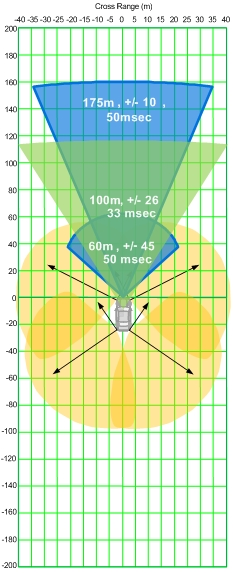
\includegraphics[width=5cm]{sensor_plan.jpg}\label{sf1}}
  \quad
  \subfigure[][传感器CAN总线拓扑]
  {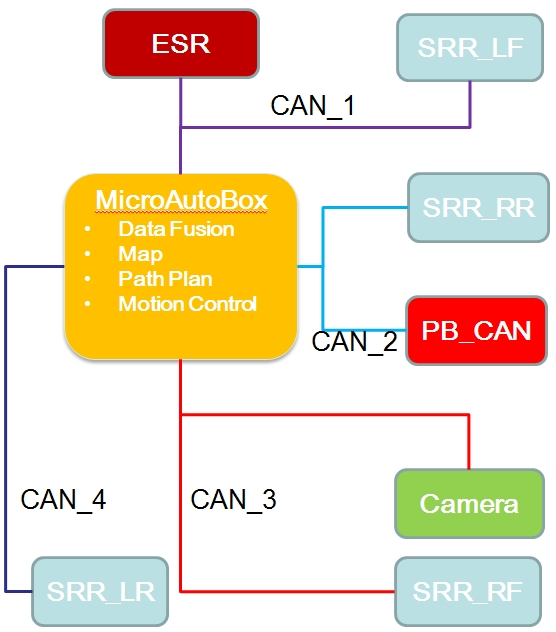
\includegraphics[width=6cm]{bus_topo.jpg}\label{sf2}}
  \caption{传感器方案图\parencite{WangZihan2017}}
\end{figure}

%%%%%%%%%%%%%%%%%%%%%%%%%%%%%以上为论文引言部分%%%%%%%%%%%%%%%%%%%%%%%%%%%%%%%%%%%%%%%%%%

% \color{}
% {\zhiv{\song{

%%%%%%%%%%%%%%%%%%%%%%%%%%%%%以下为论文第二部分%%%%%%%%%%%%%%%%%%%%%%%%%%%%%%%%%%%%%%%%%%
\section{\textbf{\song{\zhiv 基于静态离线地图的目标定位和融合}}}
\begin{figure}[!htb]
  \centering
  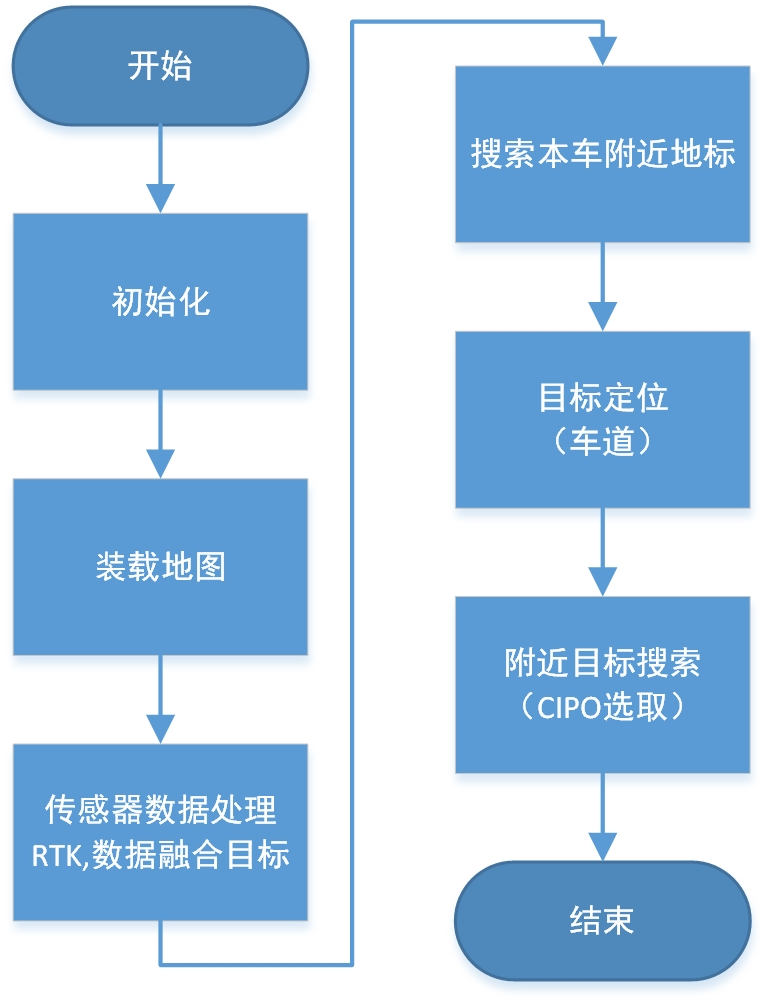
\includegraphics[width=200pt]{mapping_flowchart.jpg}
  \caption{基本算法流程图  \label{f_basic_algo_flowchart}}
\end{figure}
本方案是基于静态采集的地图结合实时RTK信号来实现车辆和目标定位。基本算法流程如 图\ref{f_basic_algo_flowchart}
\begin{figure}[!htb]
  \centering
  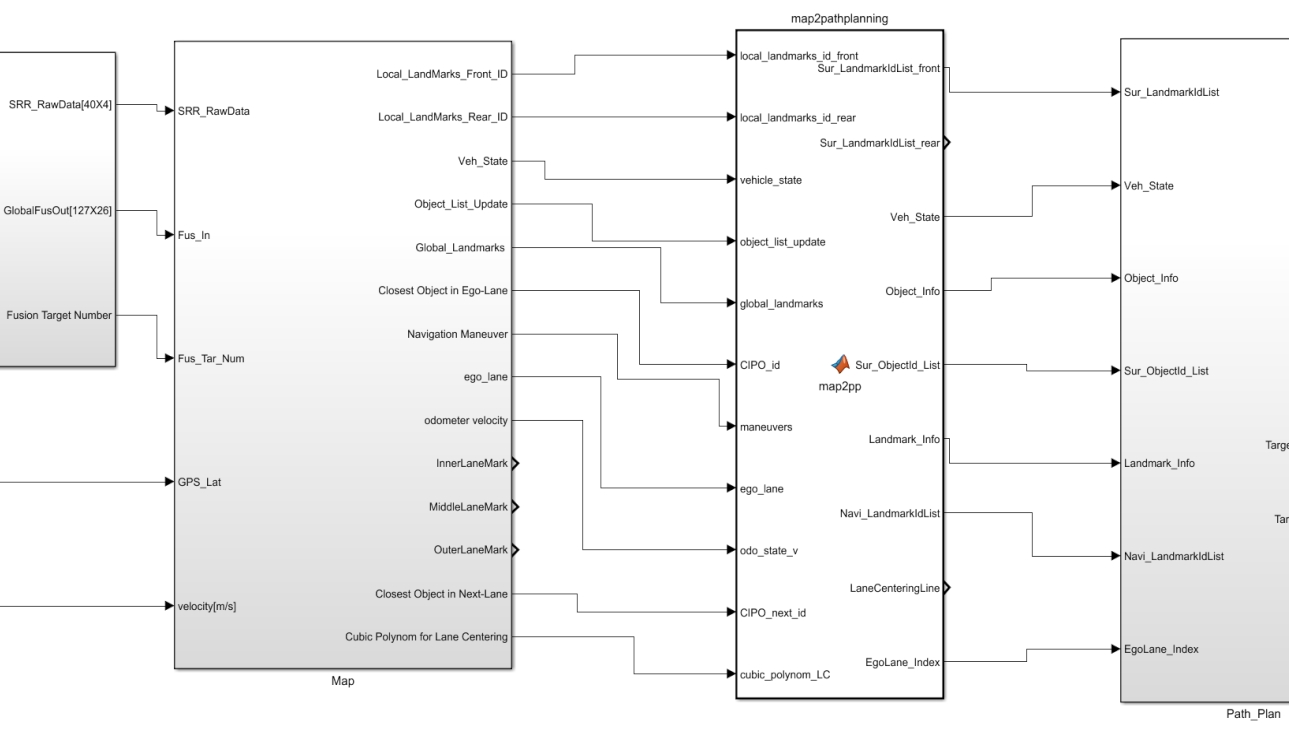
\includegraphics[height=250pt]{model_main.jpg}
  \caption{仿真环境Simulink模型\label{f_model_main}}
\end{figure}

在仿真及实时Autobox环境中的接口如图\ref{f_model_main}
\begin{figure}[!htb]
  \centering
  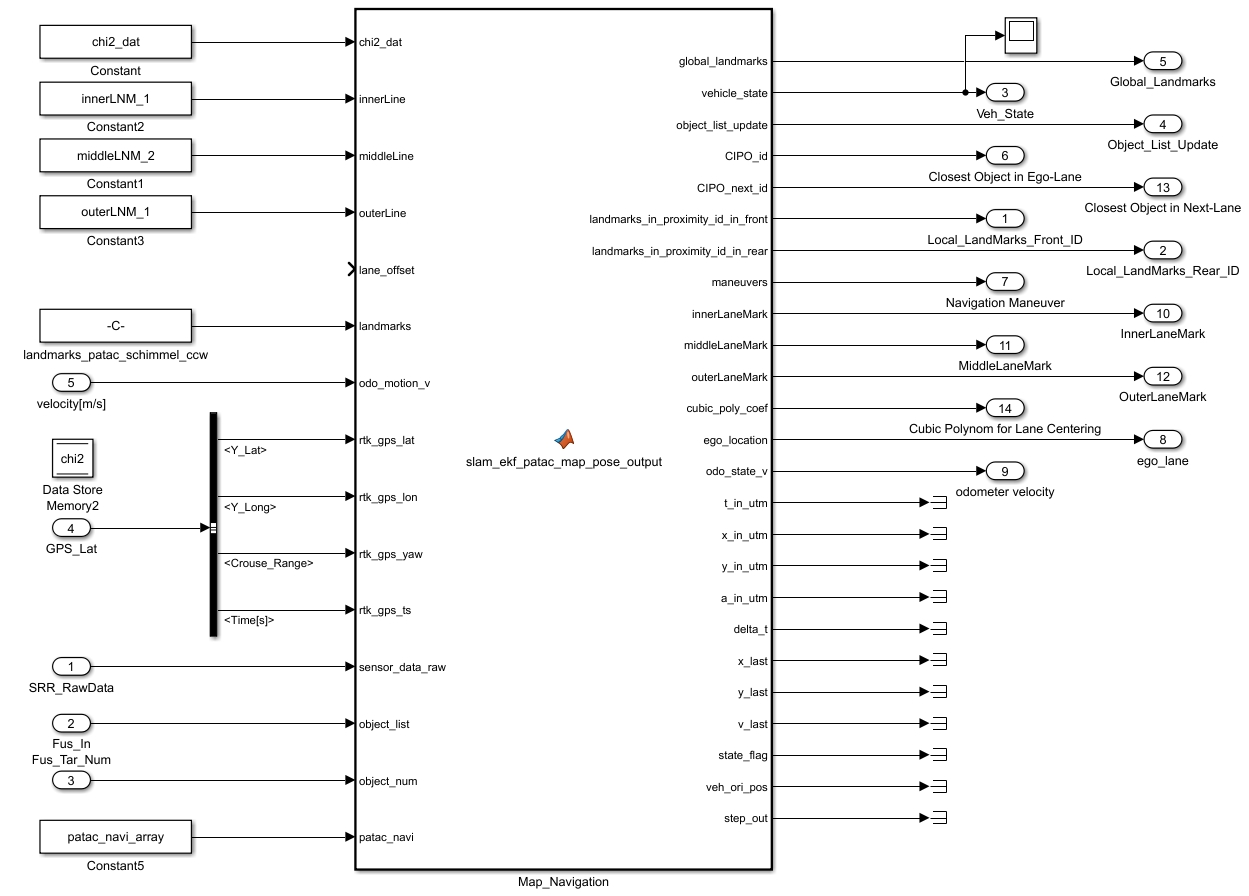
\includegraphics[height=300pt]{model_mapping.jpg}
  \caption{地图模块Simulink模型\label{f_model_mapping}}
\end{figure}

地图模块的Simulink模型及接口如图\ref{f_model_mapping}

\subsection{\textbf{\song{\zhiv 静态地图采集和存储}}}
静态地图是车道线和地标的集合。此处地标主要包括限速标志,停止线,人行横道线等。
本项目园区道路是由道路分隔线,路边沿组成的;地标有如下种类。
\begin{minted}[linenos]{c}
enum LandMarks{
// 十字路口停止线
    XCrossing_Stop = 11,
// 十字路口目标车道进入线
    XCrossing_Start = 12,
//T字路口停止线
    TCrossing_Stop = 21,
//T字路口目标车道进入线
    TCrossing_Start = 22,
//人行横道线
    ZCrossing = 30,
//边线1(沿车道横向边线),摆渡车停车点。
//停车点可能没有实际的标记,请按估计的停车点选取位置,
//比如添加2号楼门口的停车点
    Stop_1 = 51,
//边线2(沿车道横向边线)
    Stop_2 = 52,
// 左转L形路口停止线
    LeftTurn_Stop = 61,
// 左转L形路口进入线
    LeftTurn_Start = 62,
// 右转L形路口停止线
    RightTurn_Stop = 71,
// 右转L形路口进入线
    RightTurn_Start = 72,
// 路边停车位边线1(沿车道横向边线)
    ParkSlotOnRoad_Stop = 81,
// 路边停车位边线2(沿车道横向边线)
    ParkSlotOnRoad_Start = 82,
//  路外停车位,只需测量沿道路行驶方向的开始点和停止点
    ParkSlotOffRoad = 90,
//  路外停车位,只需测量沿道路行驶方向的开始点
    ParkSlotOffRoad_Start = 91,
//  路外停车位,只需测量沿道路行驶方向的停止点
    ParkSlotOffRoad_Stop  = 92,
// 车道宽度变化点,如两点间距离暗示车道宽度,
//则此时两点选取应保证,两点连线同测量处的车道垂直,
//或者增加车道宽度的域。
    RoadChange = 100,
//限速标志,点类型
    SpeedLimit = 110,
//地上箭头(参考EPM3的箭头位置定义),点类型
    GroundArrow = 120,
//交通灯位置,点类型
    TrafficLight = 130,
//其他
    UnClassified = 180,
}
\end{minted}
地标分三类,点,线和面。所有地标统一主要由两对浮点数和类型值构成。如果两对浮点数相等的,表示点地标。线地标的两对浮点数表示线段的起点和终点。面坐标有Bounding Box的两个对角顶点描述。 车道线用位于线上顺序的点序列描述。

车道线与路沿采集都由RTK设备离线采集。由于采集到的点是GPS的经纬度信号,需要转化为量纲为米的长度单位,这里的转换是从地理坐标系到局部坐标系,有Mercator变换完成。

图\ref{sf1_map}显示的是用RTK设备采集的车道线和地标。图\ref{sf2_osm}是对应的园区卫星图\parencite{OpenStreetMap} 。

\begin{figure}[!htb]
  \centering
  \subfigure[][地标及车道线]
  {\includegraphics[width=20cm]{map.jpg}\label{sf1_map}}
  \quad
  \subfigure[][OpenStreetMap园区卫星图]
  {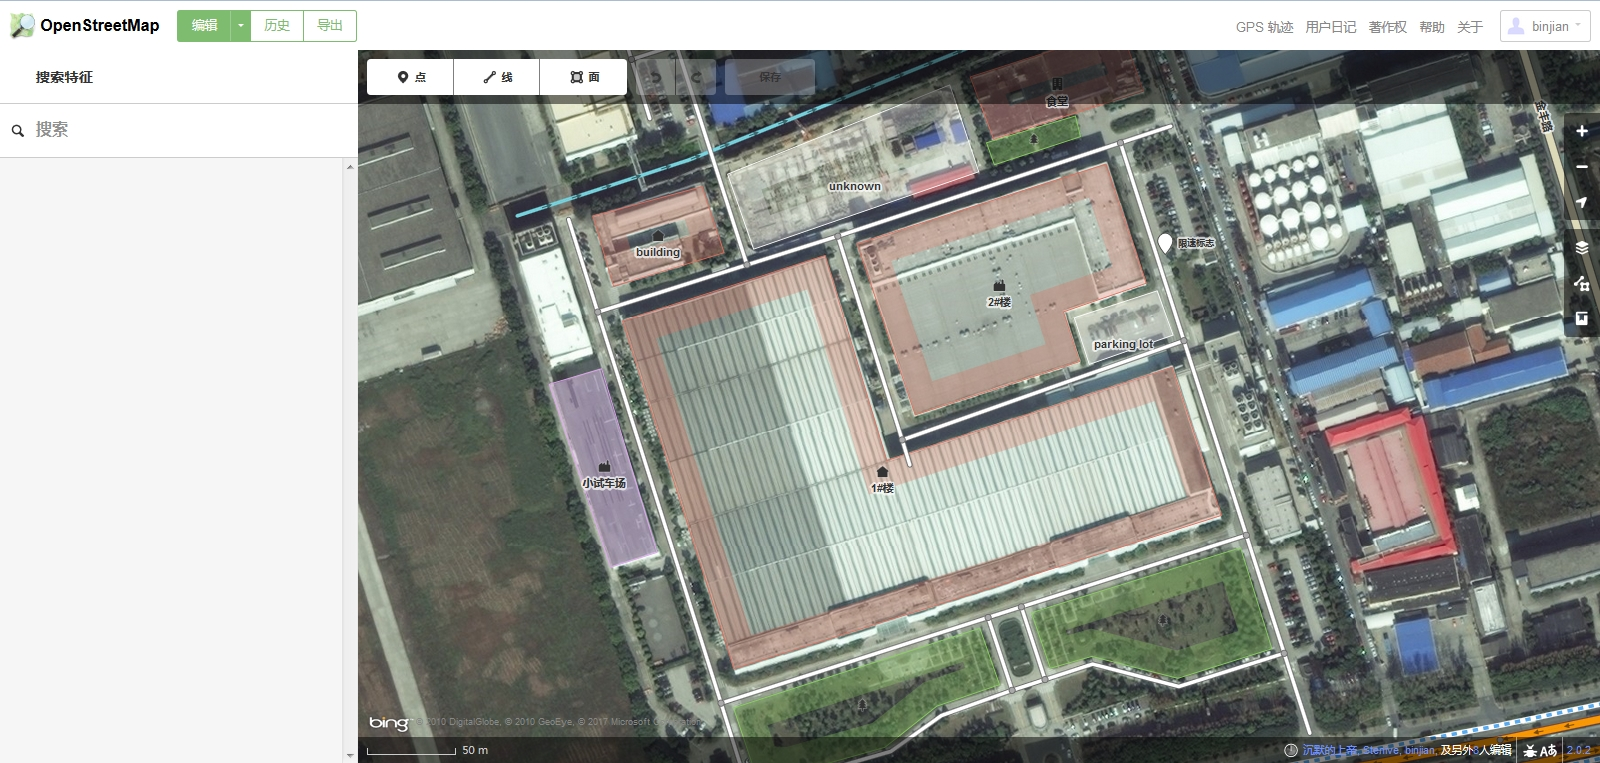
\includegraphics[width=16cm]{osm_patac.jpg}\label{sf2_osm}}
  \caption{静态全局地图 \label{f_map_landmarks}}
\end{figure}

{\subsubsection{\song{\zhiv 参考坐标系定义和转换}}}

本项目用到的坐标系有(参见图\ref{f_coordinatesystem}):
\begin{itemize}
\item 地理坐标系GCS (Geographic Coordinate System),由经纬度表示。
\item 局部坐标系LCS (Local Coordinate System),原点在地面上的选定的某个点(此处为车辆上电时的位置),正东方向为$X$轴,正北方向为$Y$轴,$Z$轴向上,旋转角正向为沿$Z$轴逆时针方向。
\item 车辆坐标系VCS (Vehicle Coordinate System) 以车辆形心为原点,车辆行驶方向为$X$轴,垂直行驶方向向左为$Y$轴,$Z$轴向上。
\item 传感器坐标系SCS (Sensor Coordinate System) 以车辆前保险杠中点为原点,坐标轴方向与车辆坐标系一致。
\end{itemize}
\begin{figure}[!htb]
  \centering
  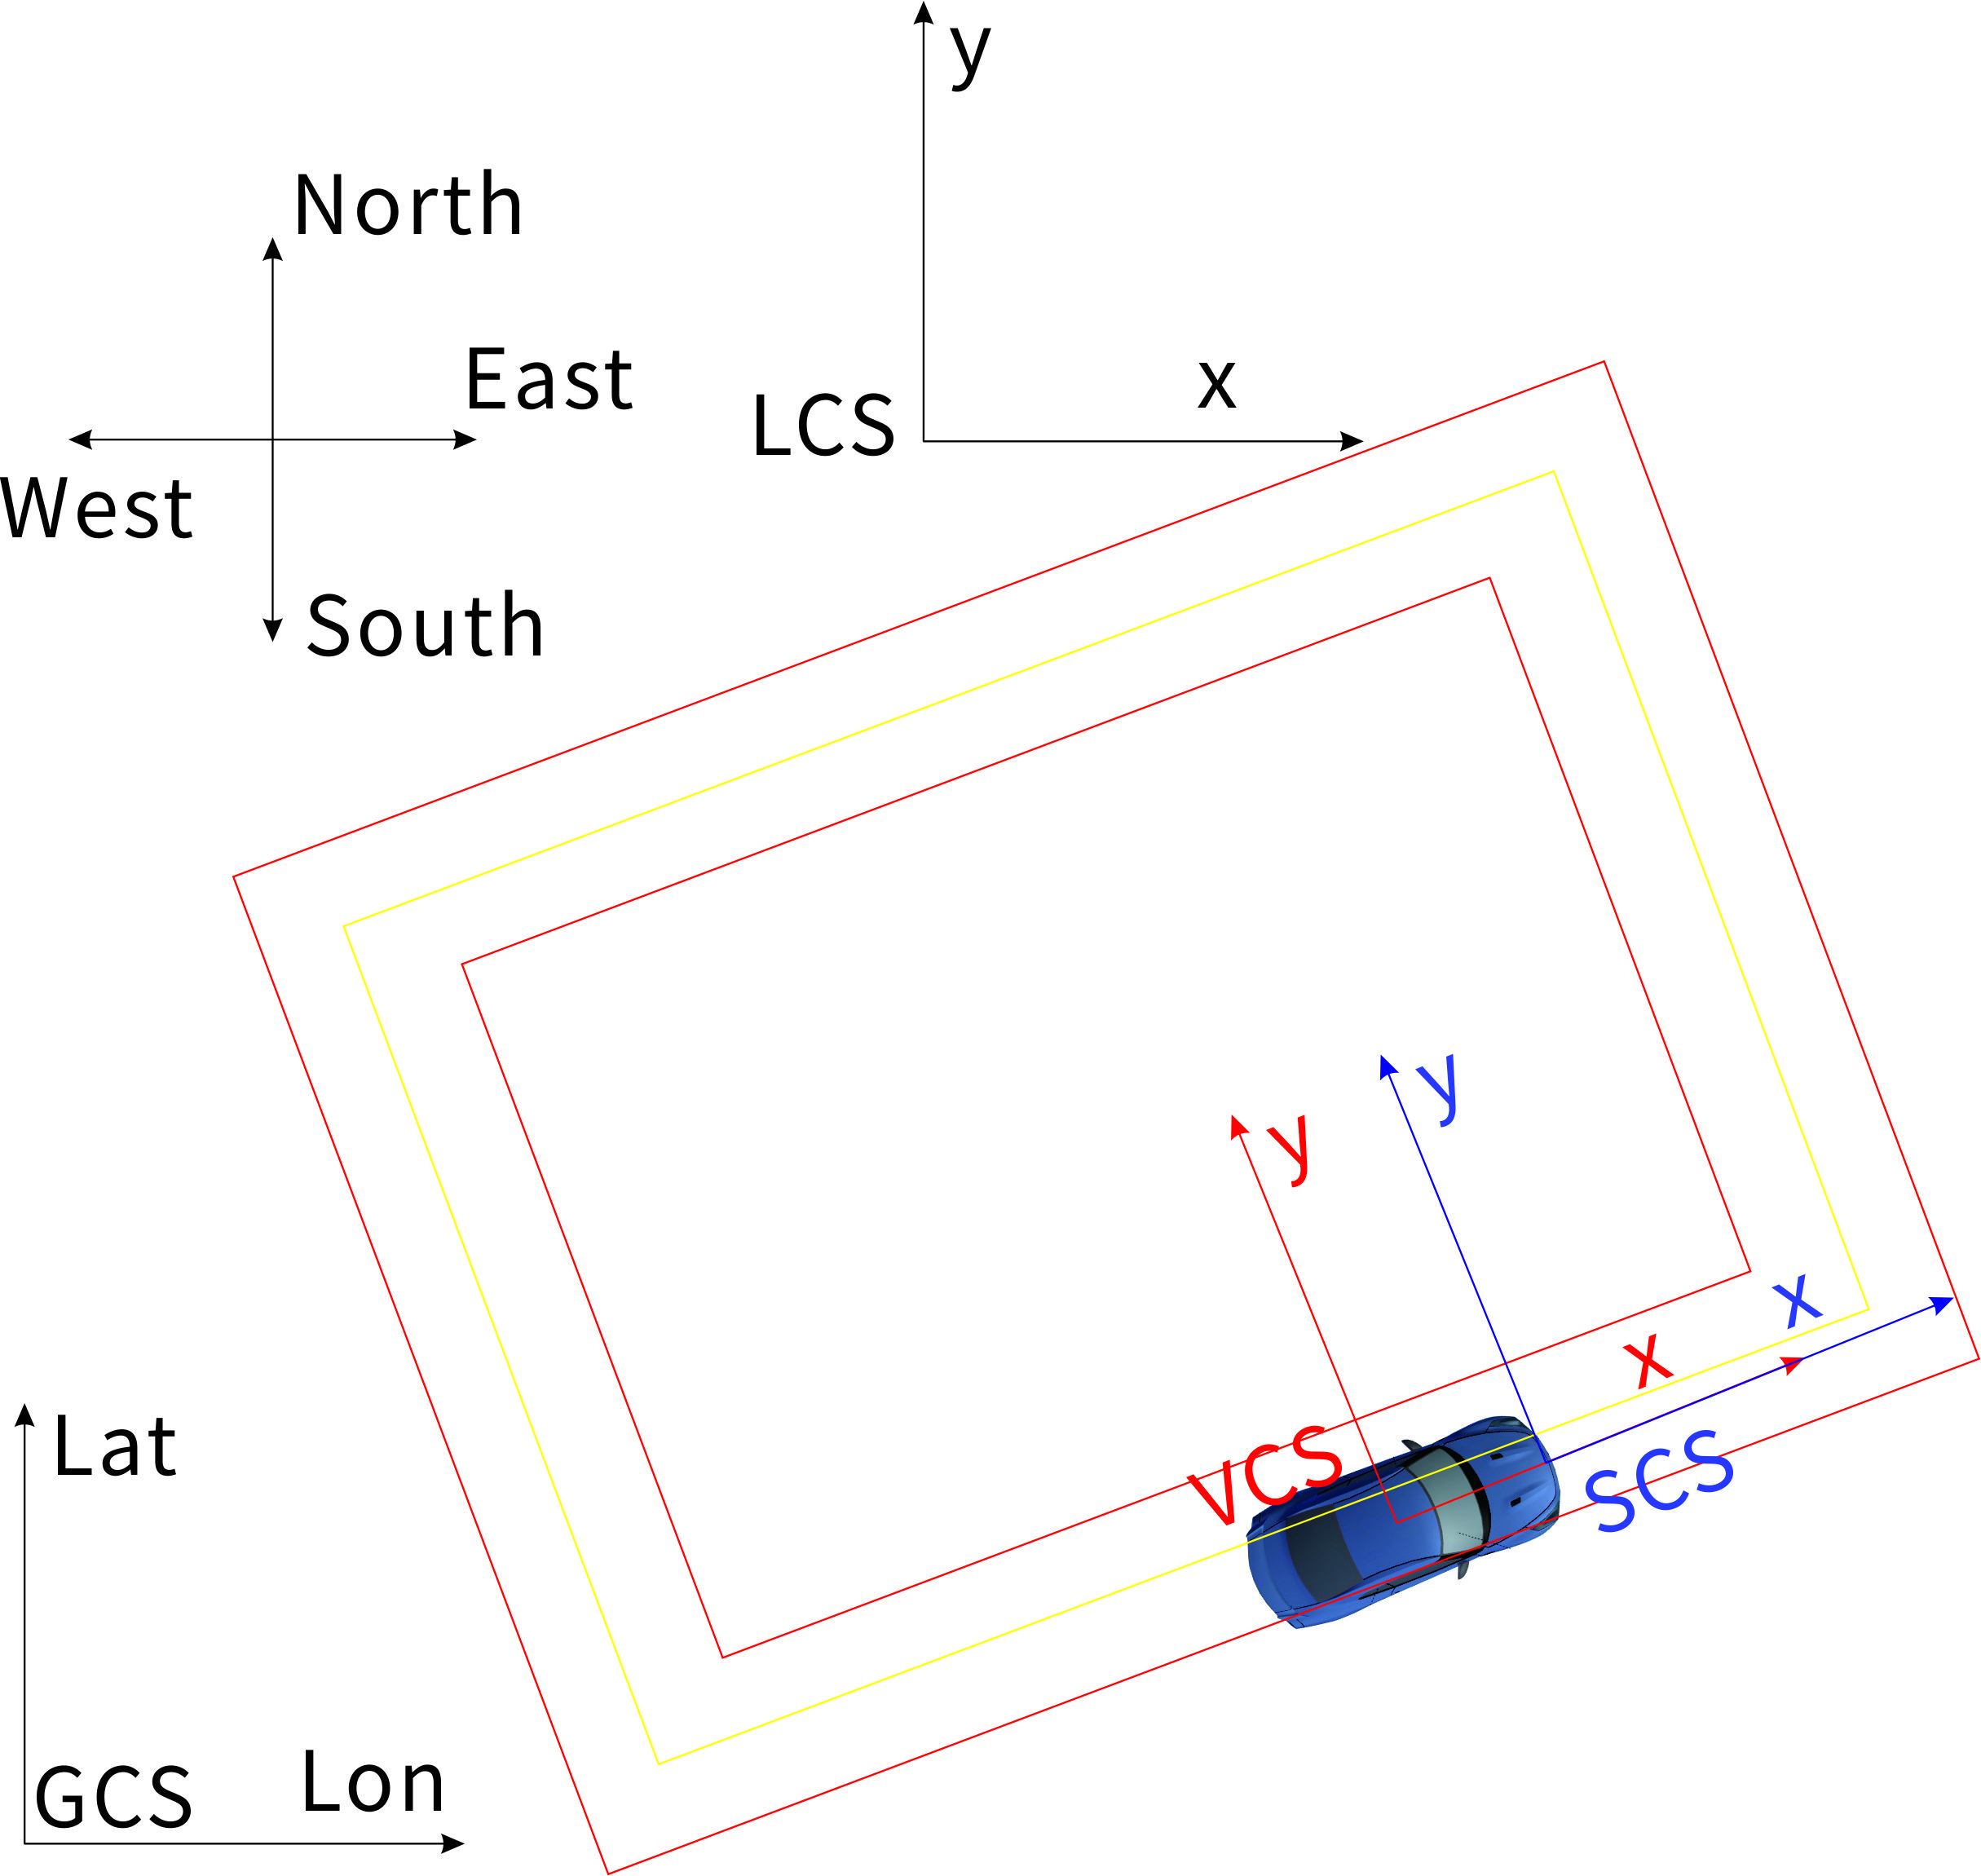
\includegraphics[height=200pt]{coordinatesystems.jpg}
  \caption{用到的坐标系 \label{f_coordinatesystem}}
\end{figure}
图\ref{f_vcs}显示了车辆坐标系。
\begin{figure}[!htb]
  \centering
  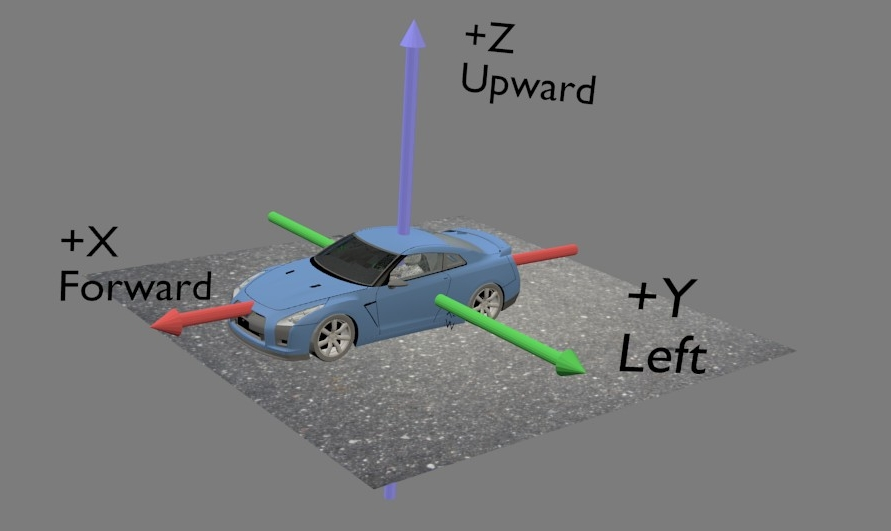
\includegraphics[height=200pt]{vcs_blender.jpg}
  \caption{车辆坐标系VCS \label{f_vcs}}
\end{figure}

\subsection{\textbf{\song{\zhiv RTK数据处理}}}
本模块用到的RTK数据有四个,经度,纬度和航向角和GPS时间。本车定位由RTK信号给出。
由于RTK信号更新周期大于与地图模块运行周期,以及由于上电导致启动不同步或者潜在建筑物遮挡导致地图模块收到无效信号,需要进行RTK信号有效性判断和相应的插值。

经纬度和Mercator坐标转换由转换函数\parencite{WGS2UTM} 完成。


\subsection{\textbf{\song{\zhiv 附近地标搜索}}}
车辆行驶过程中需要知道附近的地标信息以决定相应的行驶动作(Maneuver)。查询实时更新,由本车当前位置和本车查询范围(本车附近的搜索半径,比如50米)确定。
搜索到的地标需要进行排序,区分本车前方路标和本车后方路标并按行驶方向顺序输出。

\subsection{\textbf{\song{\zhiv 本车和目标的车道定位}}}
本车的定位由RTK实时信号确定,由于RTK输入信号周期是地图模块任务更新周期的5倍。在RTK信号更新之间的4个周期用定速和定航向角模型进行位置的插值。再结合静态地图中车道线的坐标判断本车在哪个车道,以及在车道中的位置。

数据融合的目标追踪模块的参考坐标系是传感器坐标系SCS,需要经过一个刚体变换转换到车辆坐标系,叠加RTK信号给出本车在局部坐标系中的位置,就可以得出每一个目标在车道的位置,确定所属的车道。
图\ref{f_local_map_flowchart}给出了局部地图生成和定位算法的流程图。图\ref{f_map_object}展示了本车及目标在局部地图上定位的一个结果。


\begin{figure}[!htb]
  \centering
  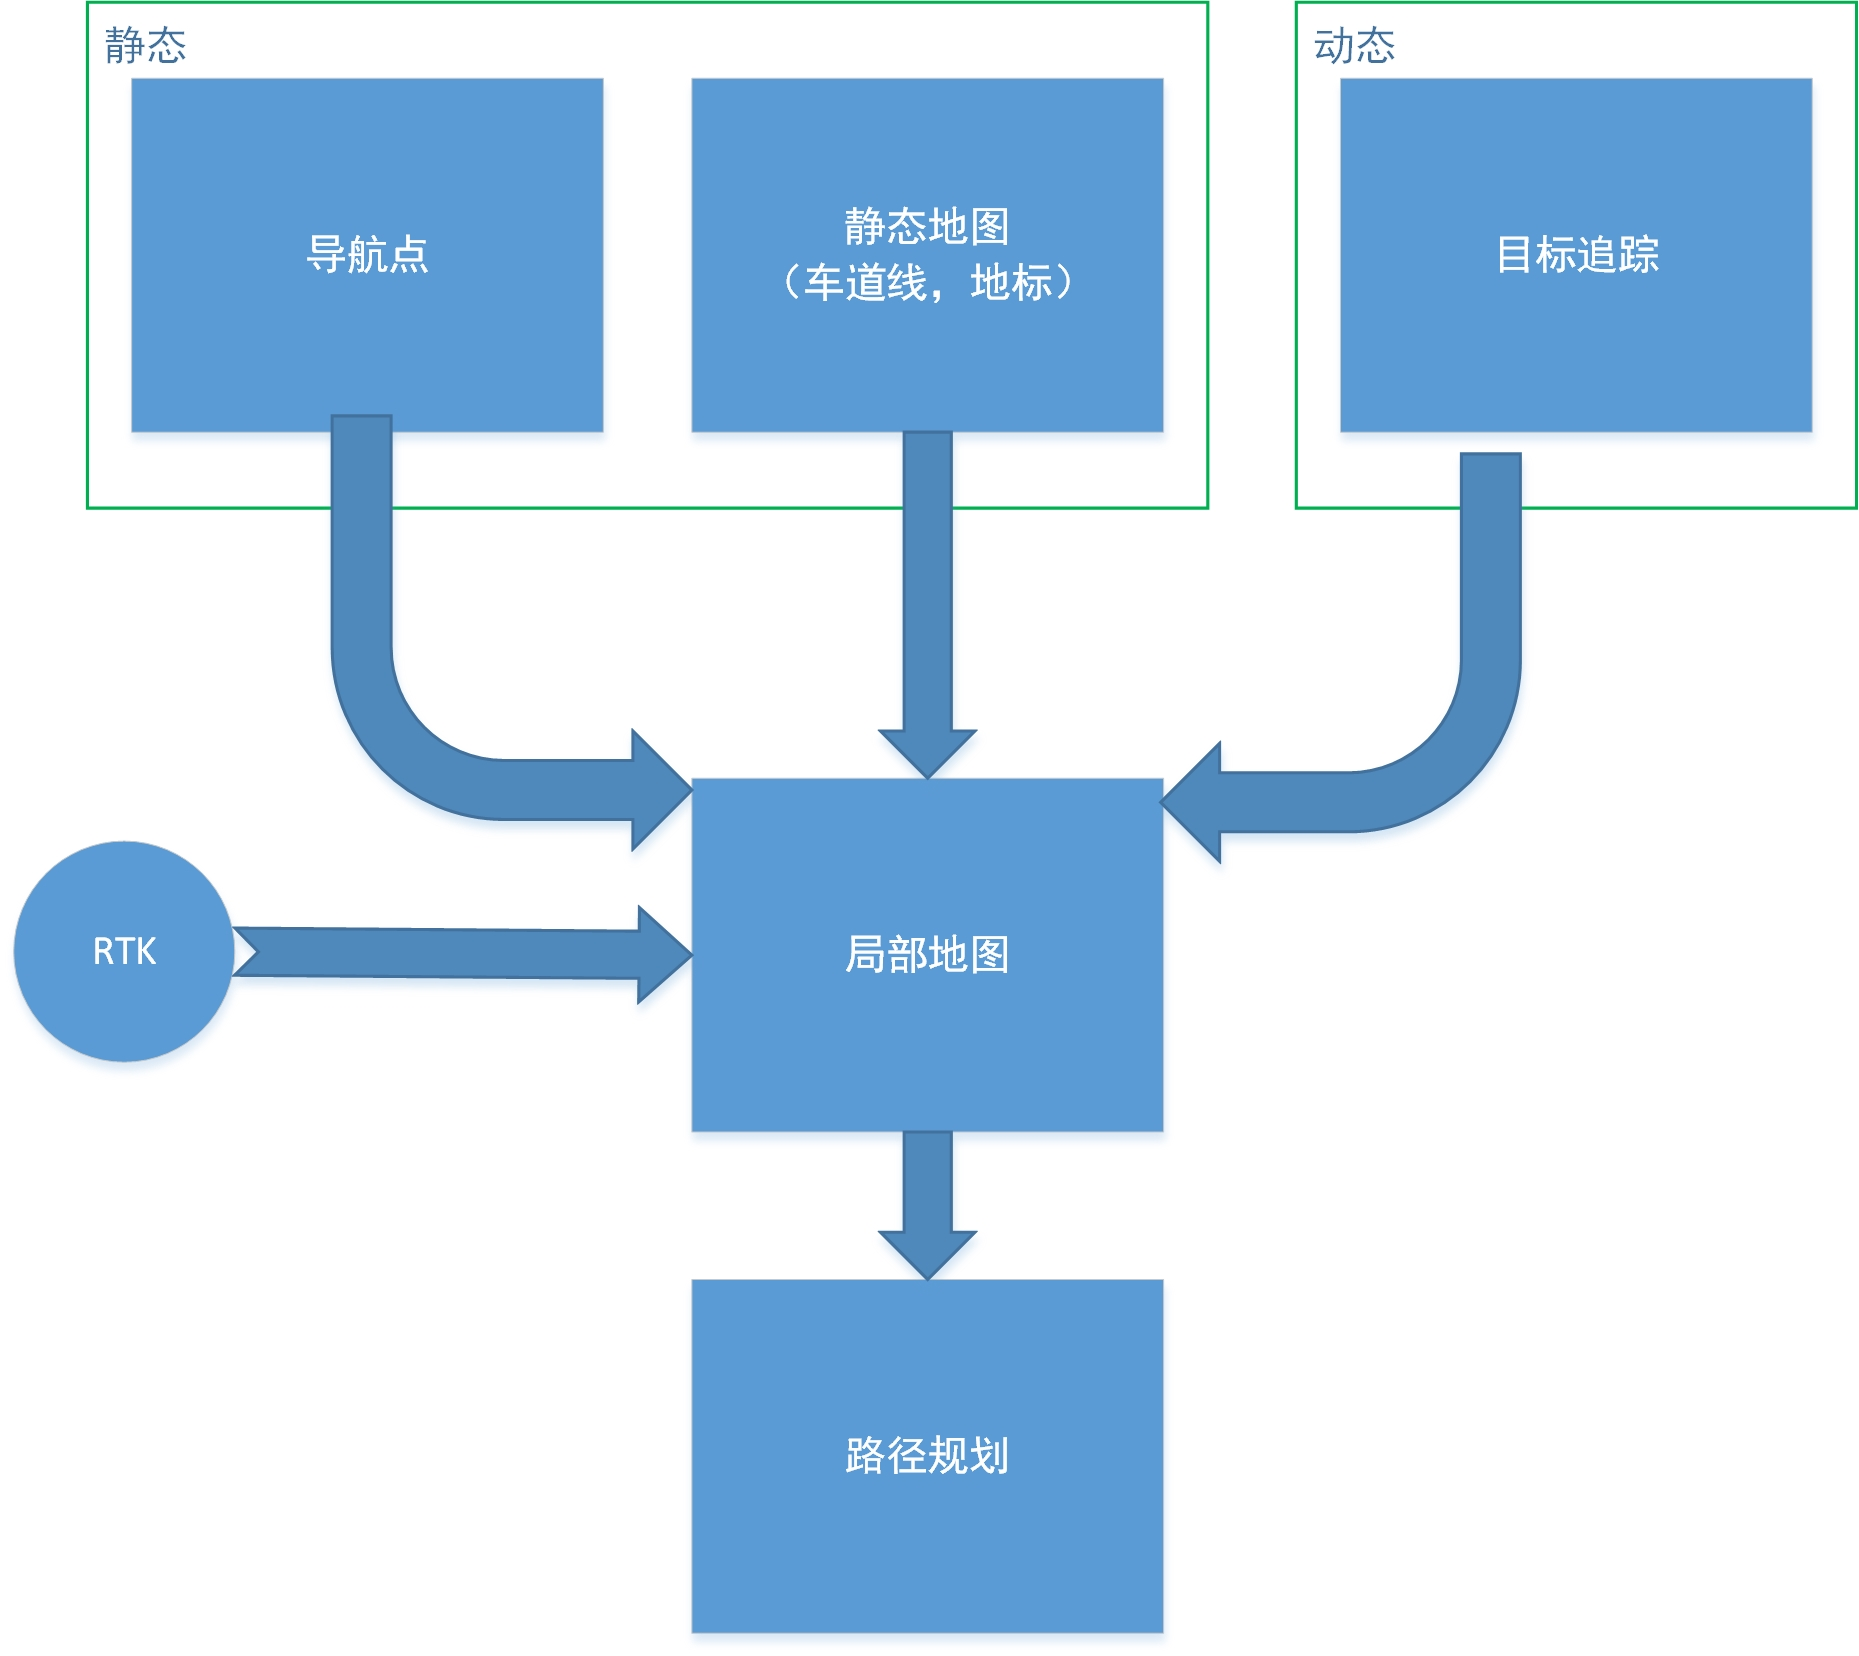
\includegraphics[width=10cm]{local_map.jpg}
  \caption{局部地图生成 \label{f_local_map_flowchart}}
\end{figure}
\begin{figure}[!htb]
  \centering
  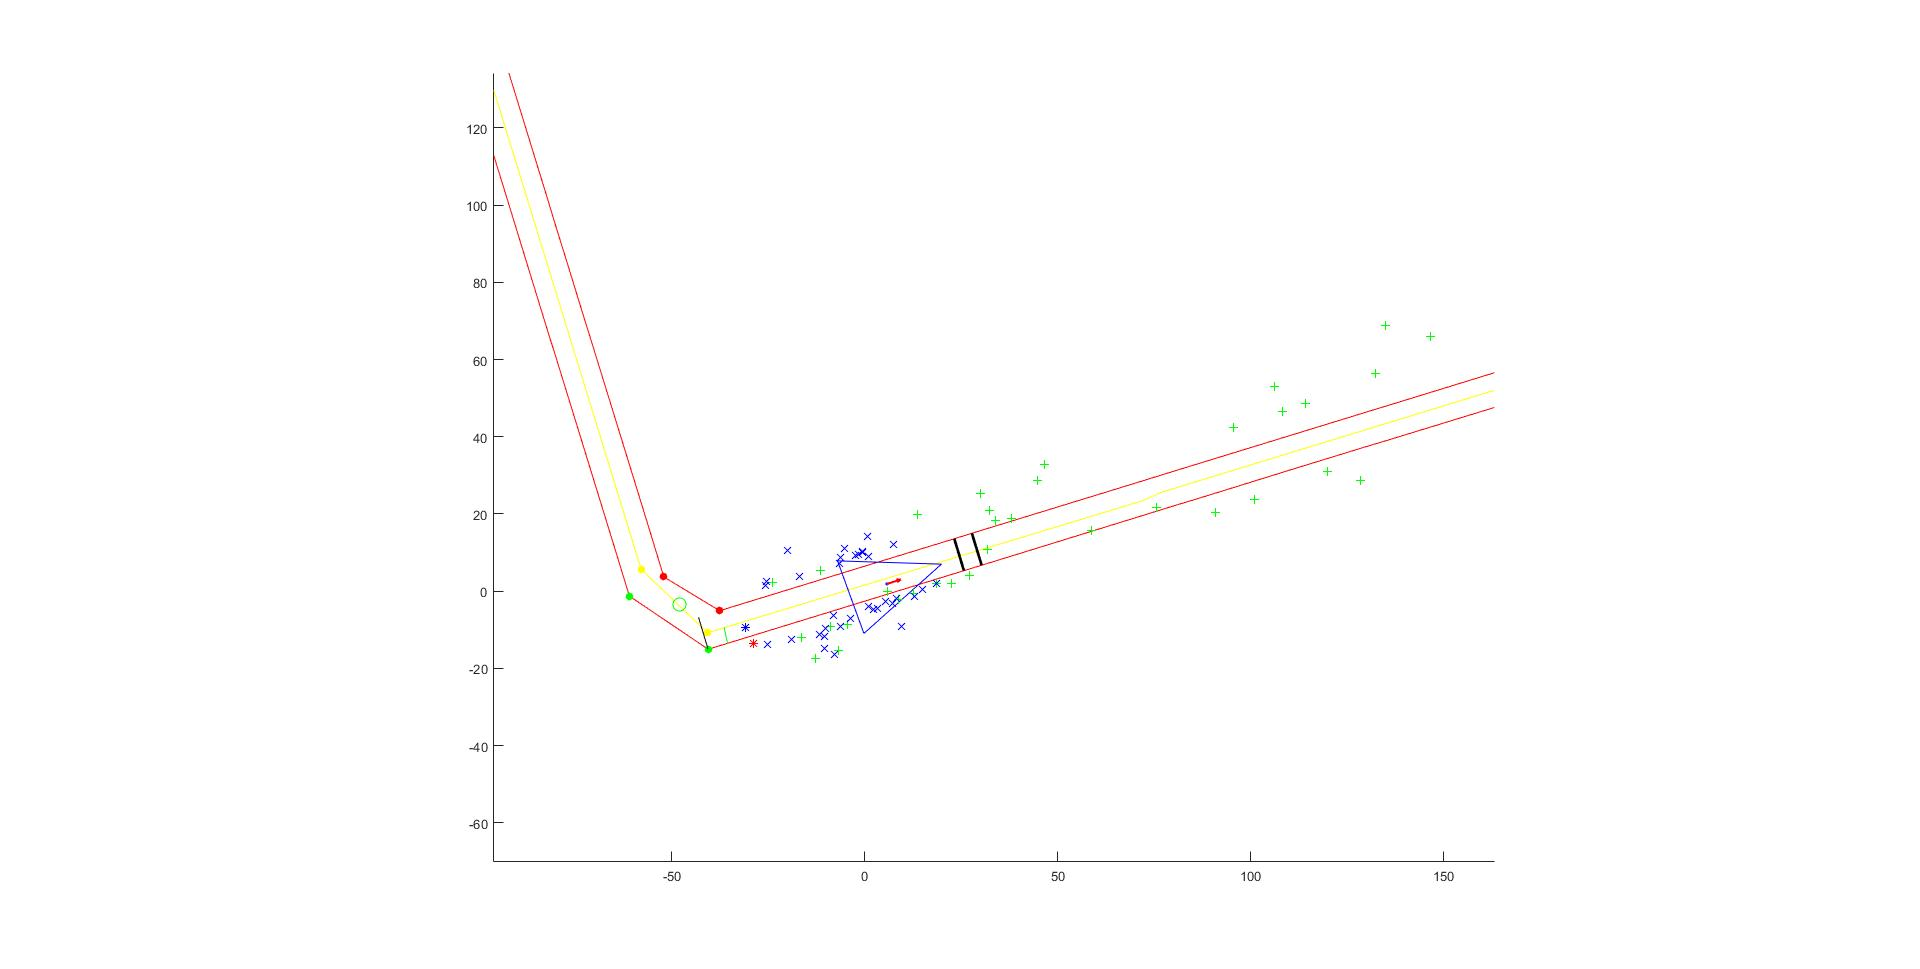
\includegraphics[width=16cm]{map_object.jpg}
  \caption{本车及目标在局部地图上的定位\label{f_map_object}}
\end{figure}

\subsection{\textbf{\song{\zhiv 附近目标搜索及最近本车道目标CIPO选取}}}
搜索本车附近的目标由两部分组成,先筛选车道上的目标,区分本车道和相邻车道的目标。然后按每个车道上目标沿车道行驶方向的纵向距离进行排序,并确定本车道最近目标(CIPO)。
排序是按车道坐标系(一维坐标系)。先将每个目标投影到车道线上,再按车道线投影的先后次序排序。

%%%%%%%%%%%%%%%%%%%%%%%%以上为论文正文第二部分%%%%%%%%%%%%%%%%%%%%%%%%%%%%%%%%%%%%%%%%%%%%%%%



\section{\textbf{\zhiv 利用SRR数据生成地图和定位 SLAM}}
地图生成和定位(SLAM)是为了解决在没有RTK定位系统的情况下,如何生成局部地图并确定本车在局部地图中的定位,\ref{f_ogm_ex}展示了一个占据格栅图的实例。通常的方法是将本车定位和地图都作为未知量来估计,并利用二者之间的关联性降低参数估计的复杂度,简化和加速计算。局部地图用地标(land mark)结合占据格栅的方式构造 \parencite{Thrun:2005:PR:1121596}。
\begin{figure}[!htb]
	\centering
	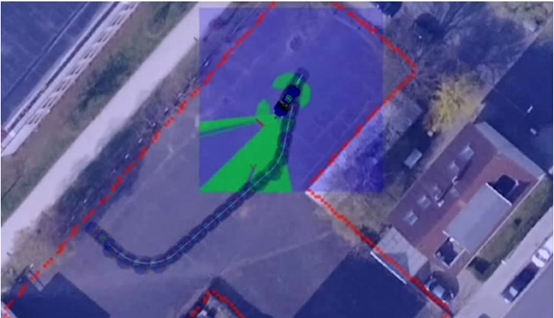
\includegraphics[height=125pt]{ogm_ex.jpg}
	\caption{占据格栅图实例\label{f_ogm_ex}}
\end{figure}

SLAM需要用到传感器的原始数据(object data),在本方案中能得到4个SRR的原始数据,所以SLAM算法的输入就是SRR的点迹数据。另外为了降低算法复杂度,区分静态和动态的目标,只考虑静态地标构成的局部地图,SRR检测出的动态目标和前置目标追踪模块给出的动态目标会叠加到局部地图上。根据静态地标占据格栅图用来更新本车姿态,目标追踪给出的动态目标通过坐标转换叠加到局部地图上。最后,静态地图和动态目标都输出给路径规划使用。

本车姿态(车辆位置,航向)和被观测目标的位置统计相关(地图,此处只考虑静态的地标),应该同时求解。当特征(地标)较少,使用基于EKF的SLAM\parencite{Castellanos2005MapBA,KF_OGM}。下面分别给出EKF-SLAM所需的世界模型,运动模型,和预测模型。

\subsection{\textbf{\zhiv 2D世界模型}}
由于传感器误差,车道线和目标追踪的结果是含有误差的,所以局部地图需要处理未知的信息以及不完全准确的定位信息。因此需要用概率的语言描述已知信息,如方程\ref{eq_ogm_prob}所示:
\begin{equation}
p(m|x_{1:t},z_{1:t})=\prod_{l=1}^L p(m_l|x_{1:t},z_{1:t})
\label{eq_ogm_prob}
\end{equation}
世界模型是以占据格栅图的形式来描述,占据和非占据信息的描述方式如图\ref{f_ogm_prob_model}所示\parencite{Elfes:1989:UOG:68491.68495}。
\begin{figure}[!htb]
  \centering
  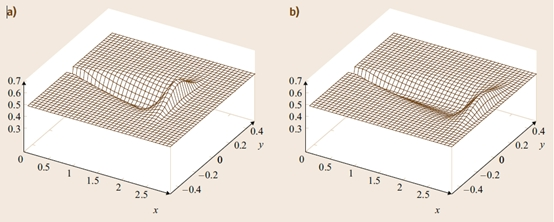
\includegraphics[height=125pt]{occupancy_prob_model.jpg}
  \caption{占据格栅图概率模型\label{f_ogm_prob_model}}
\end{figure}

{\subsection{\textbf{\song\zhiv{运动模型}}}}
\begin{figure}[!htb]
	\centering
	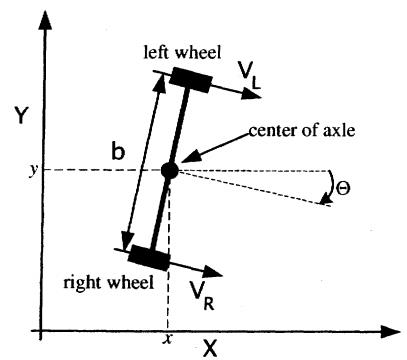
\includegraphics[height=200pt]{motion_model.jpg}
	\caption{运动模型\label{f_motion_model}}
\end{figure}

本项目使用的运动学模型如图\ref{f_motion_model}所示。运动学关系见方程组\ref{eq_motion_model}:
\begin{equation}
\begin{split}
x_{k+1} &= x_k+D_k\cdot \cos\theta_{k+1} \\
y_{k+1} &= y_k+D_k\cdot \sin\theta_{k+1}  \\
\theta_{k+1} &= \theta_{k}+\Delta\theta_{k}\\
D_k  &= v_{t,k}\cdot T\\
\Delta\theta_k  &= \omega_{k}\cdot T\\
v_{t,k} &= \frac{v_{L,k}+v_{R,k} }{2} = \frac{\omega_{L,k}R+\omega_{R,k}R}{2} \\
\omega_{k} &= \frac{v_{R,k}+v_{L,k} }{b} = \frac{\omega_{R,k}R-\omega_{L,k}R}{b}
\end{split}
\label{eq_motion_model}
\end{equation}
输入量为:
$u_k=(v_k,\omega_k)^T$
为补偿驱动轮半径不相等带来的系统误差,引入$k_1$,$k_2$和$k_3$三个参数如下\parencite{KF_OGM}
\begin{eqnarray}
\begin{split}
v_{t,k} &= \frac{k_1\cdot v_{L,k}+k_2\cdot v_{R,k}}{2}\\
\omega_{k} &= \frac{k_2\cdot v_{R,k}-k_1\cdot v_{L,k}}{k_3\cdot b}
\end{split}
\label{eq_motion_compensation}
\end{eqnarray}
方程\ref{eq_motion_compensation}取代方程组\ref{eq_motion_model}中的最后两个方程。这三个参数可以由标定来确定,不是待估计的参数。


预测方程如下:
\begin{eqnarray}
x_{k+1} &=& f(x_k,u_k,v_k)\label{eq_pred1}\\
f(x_k,u_k,v_k) &=& \left\{ \begin{array}{l}
               x_k+(D_k+v_{1,k}\cdot\cos(\theta_k+\Delta\theta_k+v_{2,k}) \\
               y_k+(D_k+v_{1,k}\cdot\sin(\theta_k+\Delta\theta_k+v_{2,k}) \\
               \theta_k+\Delta\theta_k+v_{2,k}
               \end{array}\label{eq_pred2}
               \right.
\end{eqnarray}


{\subsection{\textbf{\song\zhiv{观测模型}}}}
观测模型如图\ref{f_prediction_model}所示\parencite{EKFforLocaliOGM15}

\begin{figure}[!htb]
  \centering
  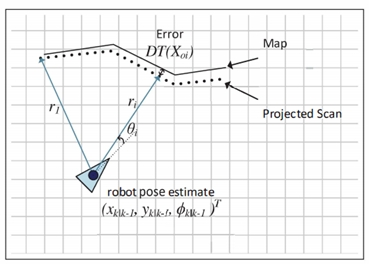
\includegraphics[height=200pt]{observation_model.jpg}
  \caption{观测模型\label{f_observation_model}\label{f_prediction_model}}
\end{figure}
此预测模型采用基于距离变换$DT$方程\ref{eq_distance_transform}的Chamfer distance $CD$方程\ref{eq_chamfer_distance}
\begin{equation}
    DT(\textbf{x}) = \min_{v_j\in V}|\textbf{x}-\textbf{v}_j|
    \label{eq_distance_transform}
\end{equation}
Chamfer distance $CD$定义如下:
\begin{equation}
h(\textbf{X},\textbf{z}) = \frac{1}{n}\sum_{i=0}^{n-1}DT(\textbf{X}_{O_i})=CD
\label{eq_chamfer_distance}
\end{equation}
其中$\textbf{X}_{O_i}$如下
\begin{equation}
    \textbf{X}_{O_i}=\begin{cases} x_{O_i} \\ y_{O_i} \end{cases} =
    \begin{cases}
    x_{k|k-1}+r_i\cos(\theta_i+\phi_{k|k-1})\\
    y_{k|k-1}+r_i\sin(\theta_i+\phi_{k|k-1})
    \end{cases}
    \label{eq_cd_x_o}
\end{equation}

最后EKF更新周期需要的隐式观测模型如下:
\begin{equation}
    h(\textbf{X},\textbf{z})
    \label{eq_implicit_observation}
\end{equation}

{\subsection{\textbf{\song\zhiv{更新}}}}
基于隐式观测模型的更新周期计算如下:
\begin{eqnarray}
K &=& P_{k|k-1} \nabla h_\textbf{X}^T (\nabla h_\textbf{X} P_{k|k-1}\nabla h_\textbf{X}^T+\nabla h_\textbf{z}^T \Sigma_\textbf{z} \nabla h_\textbf{z} )^{-1}\\
X_{k|k} &=& X_{k|k-1}+K(-h(\textbf(X)_{k|k-1},\textbf{z})) \\
P_{k|k} &=& (I-K\nabla h_\textbf{X})P_{k|k-1}
\end{eqnarray}
至此,构造了完整的EKF-SLAM的计算流程。
\section{\textbf{\song{\zhiv 附录}}}
\subsection{\textbf{\song{\zhiv 追踪列表(动态)}}}


\begin{minted}[linenos]{c}
typedef struct{
int id;
// set to 1 in the very first cycle onl that an object is output, 0 in all other cycles.
bool newObj;
//one of GCS (WGS84/UTM), LCS,  CCS, VCS, SCS, ACS, ENUM tbd
int coordinate_system;
PatObjState objState;
PatObjSize objSize;
// Pedestrian/vehicle_car/vehicle_truck/unknown/... ---> ENUM tbd.
int objClass;
//1 if the object is moving;0 if it's still;
bool moving;
//tracking when the object is seen by which exteroceptive sensor;
PatTime lastSeenBySensor[NUM_SENSOR_EXTEROCEPTIVE];
//0 for invalid; 1 for valid;
float existenceProbability;
}PatObject;

//maximally 256 tracked objects by all sensors around the vehicle;
PatObject object_list[128];
\end{minted}


{\subsection{\textbf{\song\zhiv{主控模型 m函数}}}}

\begin{minted}[mathescape,
               linenos]{matlab}
%-------------------------------------------------------
% PATAC
% ADU
% SHD
% 
% Authors:  Binjian Xin
% Date   :  11-2016
%-------------------------------------------------------
% slam, explore data association algorithms
% hd_map: offline HD map orginal ground
% odo_motion: vehicle odometer data: odo_motion.x; odo_motion.y; odo_motion.yaw;
% sensor_data_raw: raw sensor data 40x4 [ID, x, y, MoveInfo]
% sensor_data_raw.srr[4] srr(1)-srr(4) are four SRR Radar raw data.
% srr(i).Measure --> [rho tita;...]
% srr(i).Rn --> [rho tita;...]c
% sensor_data_fusion: sensor fuison data; sensor_data_fusion
% 127x26
% [ID,RangeX,VelX,RangeY,VelY,MoveInfo,Width,Type,Fus_State,Confidence,
% P11,...P44]; FuseState Byte 9 for Lane Position Judge
% hd_map offline hd map, supposed to be converted to RTM 51r : wgs2utm(Lat,Lon,51,'N');
% hd_map.lanemarking1/lanemarking2/lanemarking3: 
%            three lanes, points in counterclockwise order; 1
% for left, 2 for middle, 3 for right;
% hd_map.landmark(:,5) (x,y,length, width, LandMarkType)
% rtk_gps: rtk_gps.[lat, lon, alt, yaw, pitch, roll, ts]
% 


function [global_landmarks,...
vehicle_state, ...
object_list_update, ...
CIPO_id,...
CIPO_next_id,...
landmarks_in_proximity_id_in_front, ...
landmarks_in_proximity_id_in_rear,...
maneuvers, ...
innerLaneMark,...
middleLaneMark,...
outerLaneMark,...
cubic_poly_coef,...
ego_location, ...
odo_state_v, ...
t_in_utm,...
x_in_utm,...
y_in_utm,...
a_in_utm,...
delta_t,...
x_last,...
y_last,...
v_last,...
state_flag,...
veh_ori_pos,...
step_out] ...
= slam_ekf_patac_map_pose_output...
(chi2_dat, ...
innerLine, ...
middleLine, ...
outerLine, ...
lane_offset,...
landmarks,...
odo_motion_v,...
rtk_gps_lat, ...
rtk_gps_lon, ...
rtk_gps_yaw, ...
rtk_gps_ts, ...
sensor_data_raw, ...
object_list, ...
object_num, ...
patac_navi)
%Initialization
%...


%Convert rtk raw data to longitude, latitude, yaw in radian and ts in second
[wgs_lat,wgs_lon,wgs_yaw,wgs_ts_in_sec] = rtkraw2wgs (rtk_gps_lat,...
                                                      rtk_gps_lon,...
                                                      rtk_gps_yaw,...
                                                      rtk_gps_ts);
[x_in_utm,y_in_utm,~,~] = wgs2utm(wgs_lat,wgs_lon,51,'N');
wgs_yaw = 2*pi - wgs_yaw;


%rtk system --> VCS offset
x_rtk_offset = 0;

y_rtk_offset = 0;
a_rtk_offset = 90*pi/180;%rtk calibration info input!
x_in_utm = x_in_utm+x_rtk_offset;
y_in_utm = y_in_utm+y_rtk_offset;
a_in_utm = wgs_yaw + a_rtk_offset;
t_in_utm = wgs_ts_in_sec;

if a_in_utm>2*pi
a_in_utm = a_in_utm-2*pi;
end

chi2 = chi2_dat;
%Initialization
%Validity Check and initialization
%...


%Relocate object list in LCS
%SCS --> VCS offset 
x_scs_offset = 5.24/2.0;%vehicle length 5.24m
y_scs_offset = 0;%vehicle width 1.8m

%VCS --> CCS (Control Coordinate System) offset 
x_ccs_offset = 0;
y_ccs_offset = 0;
% x_offset = x_scs_offset+x_ccs_offset;
% y_offset = y_scs_offset+y_ccs_offset;
object_list_id = object_list(:,1);
valid = find(object_list_id);
object_num_meas = size(valid,1);

object_list_lcs = object_list;
object_num_lcs = object_num_meas;

object_loc = [object_list(1:object_num_meas,2),object_list(1:object_num_meas,4)]';
object_loc(1,:) = object_loc(1,:) + x_scs_offset;
object_loc(2,:) = object_loc(2,:) + y_scs_offset;
Tab = [ x_in_lcs; y_in_lcs; a_in_lcs];
Pa = tpcomp(Tab, object_loc);
%RangeX in LCS, displacement of VCS to SCS by 2.6m, half of vehicle length
object_list_lcs(1:object_num_meas,2)=Pa(1,:)';%object_list(:,2)+ x_scs_offset + x_in_lcs;
%RangeY in LCS
object_list_lcs(1:object_num_meas,4)=Pa(2,:)';%object_list(:,4)+ y_scs_offset + y_in_lcs;

object_vec = [object_list(1:object_num_meas,3),object_list(1:object_num_meas,5)]';
Tab = [ veh_vel(1); veh_vel(2); a_in_lcs];
Pb = tpcomp(Tab, object_vec);
%VelX
object_list_lcs(1:object_num_meas,3)=Pb(1,:)';%object_list(:,3)+ veh_vel(1);
%VelY
object_list_lcs(1:object_num_meas,5)=Pb(2,:)';%object_list(:,5)+ veh_vel(2);    

raw_loc = [sensor_data_raw(:,2),sensor_data_raw(:,3)]';
Tab = [ x_scs_offset + x_in_lcs; y_scs_offset + y_in_lcs; a_in_lcs];
Pa = tpcomp(Tab, raw_loc);
sensor_data_raw_lcs = sensor_data_raw;
%RangeX in LCS, displacement of VCS to SCS by 2.6m, half of vehicle length
sensor_data_raw_lcs(:,2)=Pa(1,:)';
%RangeY in LCS
sensor_data_raw_lcs(:,3)=Pa(2,:)';

%find local landmarks
option.firstTime=1;
option.clockWise=0;  %0 for counter-clockwise,1 for clockwise    
[landmarks_in_proximity_id_in_front_lcs, landmarks_in_proximity_id_in_rear_lcs] = ...
              quest_map4landmark_new_lane (x_in_lcs, y_in_lcs, landmarks_lcs,...
                                           middleLine_lcs.coordinate(:,1:2),...
                                           middleLine_lcs.Vertex_index,...
                                           configuration,...
                                           option);



%locate objects in lanes    
%decide object list location in lanes
option.firstTime=1;
option.clockWise=0;  %0 for counter-clockwise,1 for clockwise
object_list_update_lcs  = object_localization(object_list_lcs, object_num_lcs, ...
    innerLine_lcs.coordinate,innerLine_lcs.Vertex_index,...
    middleLine_lcs.coordinate(:,1:2),middleLine_lcs.Vertex_index,...
    outerLine_lcs.coordinate,outerLine_lcs.Vertex_index,...
    lane_offset, option);


%find the closest object in ego lane (probably CIPO)
option.firstTime=1;
option.clockWise=0;  %0 for counter-clockwise,1 for clockwise    
[obj_closest_in_path_ID, obj_closest_in_next_path_ID,ego_location_lcs] = ...
    objects_of_interest_fast(...
        object_list_update_lcs,object_num_lcs,...
        x_in_lcs, y_in_lcs, innerLine_lcs.coordinate, innerLine_lcs.Vertex_index,...
        middleLine_lcs.coordinate(:,1:2), middleLine_lcs.Vertex_index,...
        outerLine_lcs.coordinate, outerLine_lcs.Vertex_index, option);
        obj_in_path_size = size(obj_closest_in_path_ID,1);
if(~isempty(obj_closest_in_path_ID))
  CIPO_id_lcs = zeros(10,1);
  if(obj_in_path_size<=10)
    CIPO_id_lcs(1:obj_in_path_size,1) = obj_closest_in_path_ID(1:obj_in_path_size,1);
  else
    CIPO_id_lcs(1:10,1) = obj_closest_in_path_ID(1:10,1);
  end
end
obj_in_path_size = size(obj_closest_in_next_path_ID,1);
if(~isempty(obj_closest_in_next_path_ID))
  CIPO_id_next_lcs = zeros(10,1);
  if(obj_in_path_size<=10)
    CIPO_id_next_lcs(1:obj_in_path_size) = ...
        obj_closest_in_next_path_ID(1:obj_in_path_size,1);
  else
    CIPO_id_next_lcs(1:10,1) = obj_closest_in_next_path_ID(1:10);
  end
end
point_num = 30;
right_shift = 2; %counter-clockwise right shift 2m for outer lane; left shift for inner lane.
cubic_poly_coef_lcs = lanefit(vehicle_state, option.clockWise, middleLine_lcs, ...
                               outerLine_lcs, right_shift, ego_location_lcs, point_num);
%Output
%...
\end{minted}


%%%%%%%%%%%%%%%%%%%%%%%%%以下是参考文献%%%%%%%%%%%%%%%%%%%%%%%%%%%%%%%%%%%%%%%%%%%%%%%%

\clearpage %双面打印(openright) 用\cleardoublepage
\printbibliography[title={参考文献},heading= bibnumbered]
\end{document}